\documentclass[12pt]{article}    
\usepackage{ucs} 
\usepackage[utf8x]{inputenc}
\usepackage[russian]{babel}  
\usepackage{float}
\title{Псевдоэксперимент №4}
\author{Хафизов Фанис}
\usepackage[pdftex]{graphicx}
\usepackage{multirow}

\begin{document}
	\begin{figure}
		\centering
		
\includegraphics[width=0.3\linewidth]{logo}
	\end{figure}
	\maketitle
	\newpage
	\section{Зависимость $\alpha(M)$}
	$$sin(\alpha)=\frac{h}{l}$$
	$$M = mgx\cdot cos(\alpha)=mgx\cdot cos(arcsin(\frac{h}{l}))$$
	Построим график зависимости $\alpha(M)$.
	\begin{figure}[H]
		\centering
		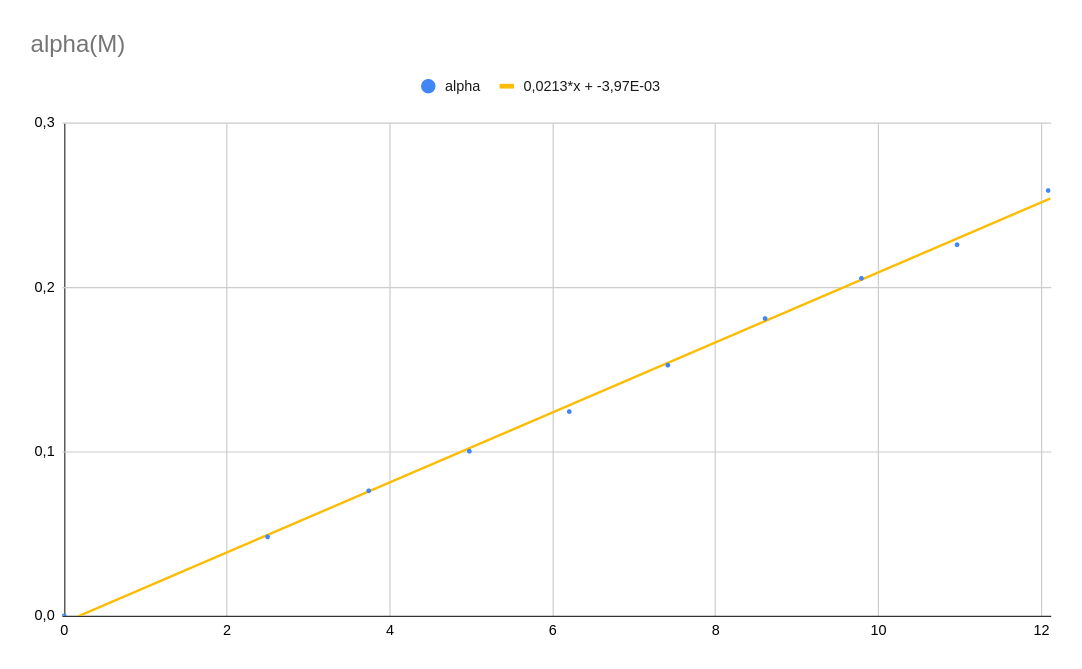
\includegraphics[width=\linewidth]{graph1}
		\caption{График зависимости $\alpha(M)$}
	\end{figure}
	По графику можно сказать, что зависимость $\alpha(M)$ линейна, то есть коэффициент $p=1$.
	\section{Зависимомть $\alpha(L)$}
	Построим график зависимости $\alpha(L)$.
	\begin{figure}[H]
		\centering
		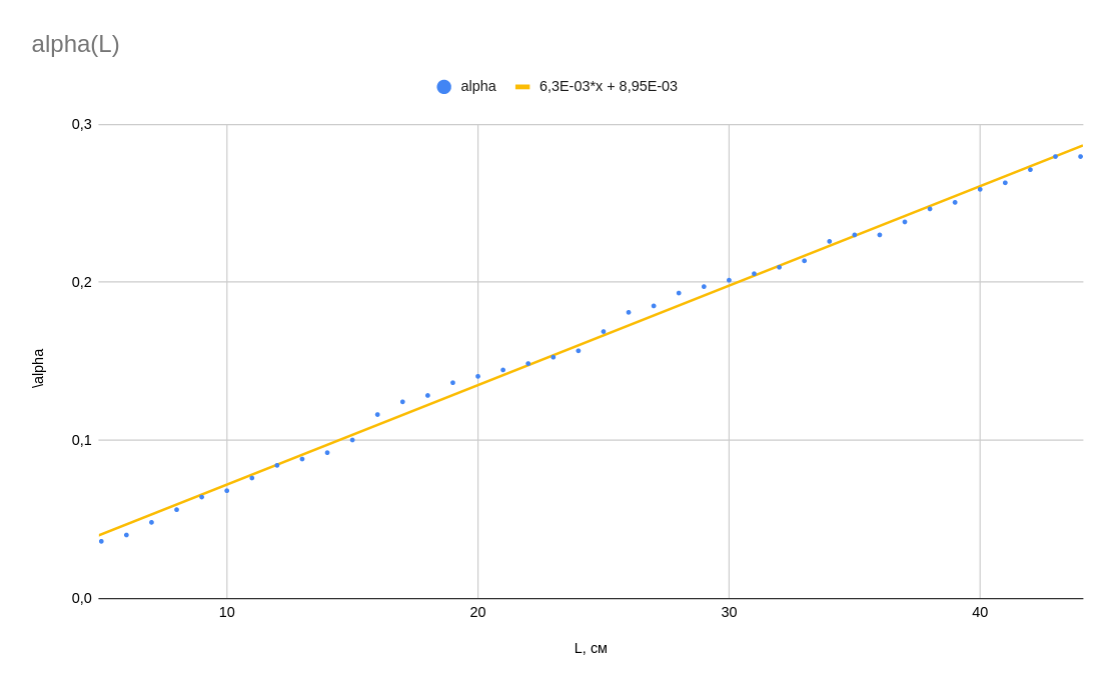
\includegraphics[width=\linewidth]{graph2}
		\caption{График зависимости $\alpha(L)$}
	\end{figure}
	По графику можно сказать, что зависимость $\alpha(L)$ линейна, то есть коэффициент $n=1$.
	\section{Определение коэффициентов $k$ и $m$}
	Так как $\alpha$ - угол, то он является безразмерной величиной. Откуда $\displaystyle\frac{6}{d}G^ka^mL^nM^p$ также безразмерная величина.
	$$[L^nM^p] = m^1 \cdot (kg\frac{m^2}{s^2})^1=\frac{kg\cdot m^3}{s^2}$$
	$$\displaystyle[\frac{6}{d}G^ka^m]=m^{-1}\cdot (\frac{kg}{m\cdot s^2})^k\cdot m^m=\frac{m^{m-k-1}\cdot kg^k}{s^{2k}}$$
	$$\displaystyle[\frac{6}{d}G^ka^m]\cdot[L^nM^p]=\frac{m^{m-k-1}\cdot kg^k}{s^{2k}}\cdot\frac{kg\cdot m^3}{s^2}=kg^{k+1}\cdot m^{2+m-k}\cdot s^{-2-2k}=1$$
	$$k = -1$$
	$$m = -3$$
	\section{Величина модуля сдвига $G$}
	$$\alpha(L) = \beta L = \frac{6M}{dGa^3}L$$
	$$\beta=\frac{6M}{dGa^3}$$
	$$G = \frac{6mgxcos(\alpha)}{d\cdot a^3 \beta}$$
	Так как измерения проводились при малых углах отклонения $\alpha$, \\то $cos(\alpha)\approx 1$. Тогда $\displaystyle G = \frac{6mgx}{d\cdot a^3 \beta}$. Найдем значение $G$, подставив в $\beta$ угловой коэффициент второй зависимости.\\
	$\displaystyle G = \frac{6mgx}{d\cdot a^3 \beta} = \frac{6\cdot 0,05 \cdot 9,8\cdot0,2}{2,5\cdot 10^{-3}\cdot 3^3\cdot 10^{-6}\cdot 0,63}=13,8\cdot 10^6$ Па	
\end{document}